\documentclass{article}
\usepackage[top=1in, bottom=1in, left=1in, right=1in]{geometry}
\usepackage{url}
\usepackage{fancyhdr}
\pagestyle{fancy}
\usepackage{setspace}
\onehalfspacing
\usepackage{graphicx}

\lhead{Building a Reliable ISP}
\rhead{Doug Woos and Qiao Zhang}

\begin{document}

\section{Introduction}

The modern Internet is deficient in reliability, security,
customizability and evolvability. The main problem is that ISPs cannot
control end-to-end delivery of their customers nor independently
introduce new services. Under the constraint of ISPs only being able
to provide what they can guarantee themselves, our broad goal is
enable ISPs to provide end-to-end delivery and a bundle of other
crucial services to their customers. However, the first obstacle is
that ISPs are currently constrained by the design of using routers and
switches with proprietary ASICs and vendor-provided routing
protocols. Our next step is therefore to design an ISP that is more
reliable and agile.

In our model, a client will make a contract with an ISP to obtain
specific guarantees about packets it sends through that ISPs
network. Specifically, the ISP agrees to deliver packets from one
specific Point of Presence (PoP) to another. The ingress PoP could
either be the client's location or that of some other ISP with which
the client negotiated a service contract; similarly, the egress PoP
could be either the final destination for the client's traffic or some
other ISP. The crucial point is that from the ISP's perspective, it
\textbf{does not matter}. The contract it has made with the client
provides delivery guarantees only between the ingress PoP and the
egress PoP. Examples of the guarantees the ISP could provide include
promises about uptime, bandwidth, and latency; for instance, Reliable
Transit Inc. might promise the client 100 Mb/s from PoP A to PoP B
with 5 9's of uptime, with a latency between 50 and 100 ms. The client
is then responsible for stitching together a route between such ISPs.

Our goal is to implement an ISP that is capable of making such
promises to clients and then reliably routing traffic. Clients can
communicate with the ISP on the control plane and the data plane. The
control plane is used to create a contract with the ISP; a client
requests a route from PoP A to PoP B and the ISP responds with a token
that the client can attach to packets so that the ISP knows to send
them along that route. The data plane is used to actually send
packets. If a packet arrives at the ingress PoP with a token the ISP
recognizes, the ISP is responsible for routing that token to the
egress PoP.

The main challenge we face in implementing such an ISP is
fault-tolerance. Traditional ISPs are configured using the BGP
protocol, which provides edge routers with information about what the
next hop should be for a given IP address. This information changes
infrequently and propagates slowly. In contrast, our ISP needs to
configure its edge routers dynamically to provide a route servicing
each new contract. The information about which tokens map to which
routes needs to be propagated and stored at the edge nodes in a
fault-tolerant manner so that if an edge node fails the remaining
nodes are able to route client traffic correctly.

\section{Related Work}
Our work is an implementation of the model presented in the TaaS
proposal. The TaaS proposal \cite{taas} provided a simulation of
traffic flowing through reliable ISPs, but did not actually implement
such an ISP. Our contribution is to provide a working,
proof-of-concept implementation of a reliable TaaS-supporting ISP, and
to show that it is possible to get adequate performance and
reliability.

We use the Paxos protocol \cite{paxos} in order to provide
fault-tolerant replication of route data. Other projects, such as
Gaios \cite{gaios}, use Paxos to sequential consistency for data
stores. Our contribution is to apply Paxos, a well-known and arguably
well understood algorithm, to a novel use case (routing within an
ISP).

Another area of related work is in Software Defined
Networking. Systems like Frenetic \cite{frenetic} allow users to
dynamically configure switches and define routes through the network
dynamically. TaaS provides a similar flexibility for the internet as a
whole; clients can view each ISP as a switch, which will reliably
route traffic from one location to another. By stitching together a
series of these ISPs, a client can be confident that its packets will
arrive at an end host reliably and promptly.

\section{Architecture Overview}
\begin{figure}
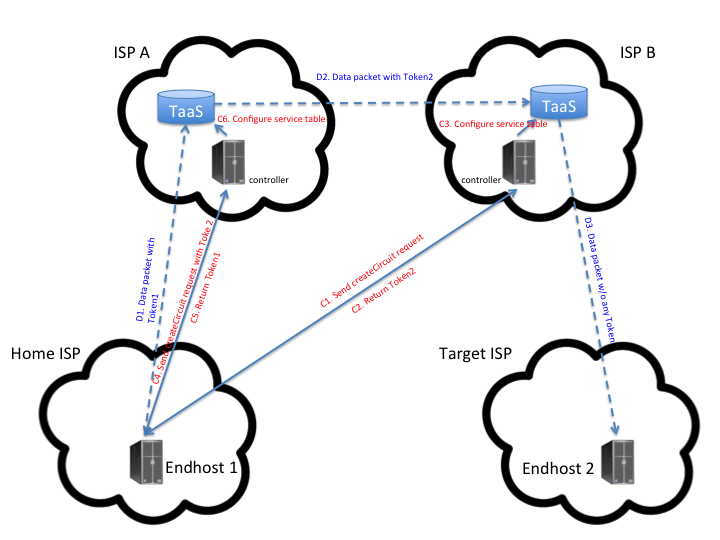
\includegraphics[width=\linewidth]{diagram}
\caption{Architecture Diagram}
\label{fig:diagram}
\end{figure}

We first describe the control plane and data plane of our ISP that
allows clients to establish circuits at various ISPs and stitch
together path segments from each ISP to forward their traffic reliably
to other end-hosts. We then describe how each ISP can maintain circuit
states in a fault-tolerant fashion. Our architecture supports an
overlay network over the IP layer that guarantees reliable end-to-end
packet delivery.

\subsection{Control Plane}

The clients can find out the costs and network guarantees provided by
a TaaS-supporting ISP through an iPlane-like service (for this
project, we assume that this is available and therefore will not
implement it). Each ISP PoP has controllers that receive requests from
clients to establish intra-domain circuits. On receiving a
createCircuit request (C1 in Figure \ref{fig:diagram}), the
controllers respond with a per-circuit-per-client authentication token
(C2) to the client. The controllers subsequently update the forwarding
tables of the Serval-supporting routers (C3) to add the new forwarding
rules in the routers (we use commodity PCs running Linux and the
Serval module to forward packets instead of dedicated routers).  The
same sequence of events (C4, C5, C6) happen for every ISP in the
circuit.

At the end of the circuit establishment phase, every ISP on the
end-to-end path will have configured the routers to have the
appropriate forwarding rules in their forwarding tables. The clients
will have a token for every circuit at every ISP that it makes
contracts with. However, since ISPs use client tokens to identify
circuits for incoming data packets, in order for clients to stitch
together circuits from different ISPs to form one end-to-end path, the
packet either has to carry all the tokens for every circuit along the
path, or the token on the packet gets modified as it exits from one
ISP and enter the next one. We adopt the second approach, and
consequently, each ISP also needs to remember the token for the next
path segment for another ISP. The createCircuit request from the
client therefore needs to contain the token for the next path
segment. The client needs to establish the whole path starting from
the last path segment entering target ISP to the first path segment
exiting the home ISP, as shown in Figure \ref{fig:diagram} and the
ordering conveyed by the sequence number of the control plane messages
(C1, C2, ..., C6). More details can be found in the TaaS paper.

\subsection{Data Plane and Stateful transformation of packets}

In order to enable each PoP to route packets through the circuit the
client purchased, we insert a TaaS-aware Serval layer in each
packet. The TaaS/Serval layer sits on top of the IP layer and below
the transport layer in the network protocol stack. The Serval header
will contain the client token that identifies the intended circuit
within the ISP. The end-hosts and each of the PoPs in a TaaS-supported
ISP will be running Serval module which allows the packet to be
transformed as it is being routed through the circuit, e.g. the PoPs
modifies the destination IP address and TaaS token of the packet as it
is routed from one hop to another. For example, as shown in the
figure, having established the circuits at each ISP, the client
(End-host 1) sends data packets with Token1 to ISP A. The routers at
ISP A use Token1 to identify the circuit the client has purchased and
forward the packets to ISP B, while changing the token to Token2. On
receiving the packet identified by Token2, ISP B routes the packet to
the Target ISP, stripping the TaaS token as the packet exits its
network.

Our ISP needs to maintain the circuit states at the control plane in a
fault-tolerant fashion. When a client requests and establishes a
circuit with any controller, we need to update and replicate the
circuit state at a group of designated nodes at the PoP. This is
coordinated using Apache Zookeeper (an open-source version of Google's
Chubby service) that uses the Paxos consensus algorithm. It ensures
that a majority of those designated nodes are aware of any given route
through the system; thus, if a node fails, the client can send traffic
through a different node. The main weakness of Paxos is its
performance cost, but as these operations are restricted to the
control plane, there is no need for them to be especially fast
(clients will send data through the system far more often than they
will request new routes).

\subsection{Failover}

Our system does not perform failure detection, since we believe that
in general the client will be able to do a better job of determining
whether its traffic is actually arriving at the server. Therefore,
failover is a client-driven process. When the client detects a
failover (i.e. it detects that its traffic is not successfully
arriving at the server), it notifies the first ISP that it believes a
problem has occured. If it does not receive an acknowledgment from the
first ISP, it concludes that that is where the failure exists and
fails over to another edge node in the same ISP. If the first ISP does
receive the client's message, it first acknowledges it so that the
client doesn't assume it has failed, then checks the second ISP in the
same way that the client checked it. Thus, the process is initiated by
the client but is actually performed at each non-failing ISP node in
the circuit.

For example, assume a circuit has been established between a client C,
ISP A, ISP B, and a server S. Each ISP has 3 routing nodes; we call
them A1, A2, A3 and B1, B2, B3. When the circuit is first established,
it goes from C to A1 to B1 to S. At some later time, B1 fails. C
detects that S isn't receiving its messages (perhaps it isn't getting
acknowledgments back). C initiates the failover process by sending a
message to A1. A1 receives and acknowledges this message, then sends a
message to B1. A1 never receives an acknowledgment, and concludes
(correctly) that B1 has failed. A1 then sends a message to B2, which
acknowledges it. A1 updates its local state so that packets on the
circuit go to B2 rather than B1, then informs the client that the
failover has succeeded. Subsequent traffic is now routed through the
new circuit.

\section{Evaluation}

The VICCI testbed consists of 4 clusters at US universities and 3
clusters at international sites. We will thus use the VICCI testbed to
implement the edge component of an ISP. Each VICCI site will function
as a PoP that the client can establish a circuit with and the PoPs
have to maintain the circuit state.  We will simulate two ISPs by
deploying our architecture on two VICCI clusters, most likely the
Stanford and Princeton clusters. At each cluster/ISP PoP, we will have
5 nodes to be the control plane that establish circuits with clients
and around 10-15 nodes to be the Serval data plane that forwards
traffic. The coordination service provided by Zookeeper will consist
of 3 nodes that may or may not overlap with the control plane nodes.

There are two goals in our evaluation. The first goal is to establish
the feasibility of stateful transformation in our ISP and evaluate the
baseline performance of our ISP in the absence of failures. We will
simulate the case where O(100) to O(1000) end-hosts establish circuits
through our ISP, and we will measure various performance metrics of
those transit circuits, e.g. bandwidth and latency. The performance
numbers will be informative of the overhead of our implementation of
the stateful transformation.

The second goal is to evaluate the fault-tolerance of our ISP. Within
the ISP, the state (the mapping from client token to the circuit the
client purchased) maintained at each PoP needs to be resilient to
failures. We model the failure of each PoP by a Poisson distribution,
and randomly choose a PoP and shut down one of the its machines. We
then measure the performance metrics with respect to such failures. In
the ideal case, if the failures are infrequent enough, we should
expect to see little degradation in the performance. We will push the
system to the extreme and establish the point at which the system
experiences severe performance degradation.

\bibliography{bibliography}
\bibliographystyle{plain}

\end{document}
